\section{Development configuration}

This project is mainly based on the JAVA programming language and the IDEs of this project are using IntelliJ IDEA. To develop a desktop application,  the java library JavaFX is utilized for building a GUI platform. Moreover, to port FXML mark-up to an IDE, Scene Builder is chosen for this project to facilitate. All the specified compiled versions of the software components are shown in Table~\ref{tab:software version} below. 

\begin{table}[h]
	\centering
	\begin{tabular}{l|r}
		\toprule
		Components & Version \\
		\midrule
		Java Development Kit (JDK) & JDK 17 \\
		Scene builder & 18.0.0 (the latest version)\\
		\bottomrule
	\end{tabular}
	\caption{A software version table.}
	\label{tab:software version}
\end{table}

\section{Problem analysis and realization}

This section presents the problem which the designer faced when he or she developed and designed the process of the game CrossWise. The problems are related to the GUI interface, the game logic design, or the necessary elements which are considered to implement. In addition, this section not only contains the analysis of the problem but also gives some specific realizations of the problems.
\newpage
\subsection{GUI representation of the game windows}
\subsubsection{Problem analysis}

Considering the fluent game-playing process, the setting of the player name or whether some AI players are participating must be decided at the beginning. Thus, how to manage those setting is an issue. There are two ways to implement it,  either in one- window or in a separate window. 

\paragraph{All in One window} \mbox{}\\

An ideal all-in-one window is that selecting the player amount and input player name can be determined in the main interface. All the possible situations for the human players and computer players are created in the menu bar by using the menu item. The advantage of this option is that all the game settings can be determined in one window. However, after during the game for a while, once users want to change their name and chooser another mode of the game, the previous setting will disappear. 

\paragraph{Tow separated windows} \mbox{}\\

An ideal of this situation is using two windows to represent the whole game running. One is for selecting the player's amount, determining the human player or the computer player, and also available to input the player's name. Another window is used to display the whole game field which is the main interface of the whole game. The first window can be invoked from the menu bar of the second game interface which named as "New game".    

\subsubsection{Realization analysis}

To solve the difficulty of switching the players' related settings, it is achievable and possible to manage all initial settings in the two windows. Here include several workable realizations below: 

\begin{enumerate}
	\item\textbf{UserInterfacePlayer.fxml}\\
    In order to initiate the player setting, an FXML interface needs to be created which means an additional scene builder has to be used. Many elements of the items will be managed properly on this scene builder, for example, GridPane, Label and CheckBox, and so on.  
	
	\item\textbf{Stage}\\
    A Stage class is used to invoke an owner window. In this problem consideration, we will use the Stage class to invoke the second window for initializing the player settings. After the player setting is done, a Stage object also will be used to switch back to the primary interface. 
	
	\item\textbf{CheckBox}\\
    According to different modes of the player setting, we need to decide which player is played by a Bot or a Human. Thus, a checkBox item can be used to determine this option. Each player has a checkBox item to let the user decide except for the first player. The first player must always be played by humans. 

	
\end{enumerate}

\subsubsection{Realization description}

The primary window has one branch from the menu bar. The one is originally responsible for the fundamental configuration (e.g., New game, save game, and close game.). The second window is invoked from the new game options. when the new game item is pressed, the second window will be shown up and replace every content of the first window. In the second interface of the players-related setting, there are four labels for four players, for example, player1, player2, player, and player4. Each label has a text field after itself, and the player's name can be input into it. The last column of this player setting has three checkboxes to decide human player or a Bot Player. During the game playing, the user can reselect the desired case from the second window. This two-separated-window setting does not increase the difficulty for the designer and even simplifies the data passing process of the players' names. 

\subsection{Passing data between two windows}

\subsubsection{Problem analysis}

The following analysis and description refer to how could the players' data be transferred from a Scene B controller to a Scene A controller which is the primary interface. To do so, two ways could be implemented. None of them is the perfect solution, but each has benefits and downsides to being considered in a different situation.

\paragraph{A class Controller } \mbox{}\\

Logically, when an FXML file is created in Scene B, the IDE automatically creates a controller with it and uses the root tag to link it together. Also, this controller can create a new instance in the B class, however, if we want to pass information to another controller. An instance must be created manually in class A which will accept the new information and use this new instance to obtain the accessibility of all public methods which is necessary to be used.  

\paragraph{The singleton pattern} \mbox{}\\

An idea of the singleton pattern is that two classes use the same instance of the singleton class. This class contains all the necessary information that needs to be passed. In other words, this singleton class has a getter and setter function that is able to get the data and also set the data for different situations. Broadly speaking, it can be treated as a database. 

\subsubsection{Realization analysis}

This project is passing information related to players. All players' data that need to be transferred is analyzed in several attributes. Those attributes can be treated as objects. A getter and setter function is important to exist and is utilized in the progress of passing data. The explanation of these two tools is described below.   

\begin{enumerate}
	\item\textbf{Controller Instance }\\
    An instance of a scene controller can be displayed as a class object. In addition, the direction of passing information can decide which controller class should obtain the instance. Normally, the class which accepts data has the demands to require this instance. 
   
    \item\textbf{Getter and Setter }\\
     Getter and setter functions are used frequently when the data is transferred. Every passing attribute needs its own getter in order to get the data. In the meantime, the setter can be utilized purposely in some situations where the attribute needs to set some value.    
     

\end{enumerate}

\subsubsection{Realization description}
Using the controller instance is a prompt instrument for transferring all needed data. Regarding all the attributes that need to be passed and updated in this project, there are only four attributes that need to consider. For instance, the players' names, the active state, and the state represent whether the player is a human or a bot and the amount number of players in a round. Broadly speaking, there is not so much information that needs to be passed. Therefore, a controller calling is thoroughly enough for these demands.



\subsection{Data structure of players' hands}

\subsubsection{Problem analysis}
The playing hand consists of four random tokens, which can be used to proceed with a game. In each round of the game, a token could be removed from the hand and another token could be added. Until the game approaches the end, each hand's total length may not remain at four. Moreover, the hand element always needs to be updated in each round, and also each token is able to be adjustably utilized. Thus, a data structure for adopting to build a hand should consider the following conditions.  

\begin{enumerate}
	
   \item Although the length of the hand is fixed in the beginning, the data structure should be able to adjust the size when the game approaches the end. 
   
   \item  A data structure should involve some characteristic that can easily access the element of the hand,  for example.,  the ability to remove, insert, and get the element from the index.

\end{enumerate}

\paragraph{Array} \mbox{}\\

An array is created to hold a fixed number of values of a single type. The length of an array is determined when the array is created. Therefore, in this case, a hand can give a fixed length to the array and put token elements into the array. However,  in this game, hand length cannot always be the same. It can be less than the original size of the array. As this situation happens, the way to solve this is that keeps the array has still existed and the empty position of the array can be assigned as null. 

In addition, A good point by using an array to construct a hand is that it is much easier to get the token element by calling the index. However, there is an issue need to be noticed. While one token element is removed from the array, the index of the removed element should be recorded in order to store put another token into it. Alternatively, there can be another way to do it every time a token is being removed and the array must be sorted. This is helpful to insert a new token at the end of the array instead of recoding the index of the removed token. 


\paragraph{LinkedList} \mbox{}\\

 A Linked list is a linear data structure in that elements are stored by using pointers. In other words, a linked list consists of several nodes, and a node contains a data field and a reference to the next node. With the help of the linked list structure, a hand can be designed as a linked list and each token is the node of the list. Each node is linked to each by using the link and reference. 

The advantage of the linked list structure is that there is no need to establish a fixed size for the linked list. The length of the linked list is relatively flexible. Nevertheless, a downside of the linked list is to access elements. If a token need to be taken and placed on the board game, it must be gotten by using a pointer from the first node of the linked list and moving down until reaching the target that is required.

\paragraph{ArrayList} \mbox{}\\

An ArrayList is using a dynamic array for storing the elements. It can be treated as a traditional array except it has no size limit. Also, the ArrayList allows random access by calling the array of the index and it also implements the List interface so the user can use the method of the List interface.

Based on the condition of the hand structure here,  those characteristics of ArrayList are fulfilled with the condition of this hand structure.    


\subsubsection{Realization analysis}
An ArrayList structure is suitable for the players' hand structure. It contains many different methods to be utilized. Here have some methods that can be used frequently in this project.
Those methods are shown and introduced below: 

\begin{enumerate}
	\item\textbf{add(int index, E element)}\\
An add() method can insert a specified element at the specified position in the ArrayList. This method can be used to add any new Token to the hand. 

	\item\textbf{remove(int index)}\\
A remove() method can remove an element at the specified position in the ArrayList. Once a token is chosen in a hand and it needs to be removed from the hand, this method can be called by giving a specific index.  
	
	\item\textbf{toArray()}\\
A toArray() method contains all of the elements in the ArrayList in proper sequence. This method is useful to check each element in an array and also can be used to display in the toString() method in order to show elements of each hand.  

\end{enumerate}

\subsubsection{Realization description}
A packed class is being created as a superclass of a hand class. In the pack class,  the ArrayList structure is being used and called in the pack's constructor. A hand class can straightly inherit all the methods including the Arraylist of the pack class. The length of the ArrayList can be passed as a parameter in a pack construe. Therefore, Every time user creates a hand object with a specific size of the ArrayList. Once the game happens near the end, a length size can be decreased from the parameter of the constructor to create a new array list.  
 


\subsection{A moving animation for board}

\subsubsection{Problem analysis}

Considering that the game can be played with all AI players, the running time of the whole game is considerably fast and uninterrupted. Hence, in order to slow down the whole running process for the whole game, completing a token action and utilizing an animation is considered. 

Indeed, there are some possible animation types that can be utilized, The following description explains two different kinds of animation that are being considered.  

\paragraph{Translate Transition} \mbox{}\\

The TranslateTransition is represented by the class javafx.animation.TranslateTransition. It can translate the node from one position to another position depending on the specified duration. Those positions are defined by providing the translateX and translateY properties of the node. Also, the speed of the transition can be specified by the user. 

\paragraph{Fade Transition} \mbox{}\\
In JavaFx, the class javafx.animation.FadeTransition represents FadeTransition. It animates the opacity of the node so that the image color of the node becomes dull. Also, the specified duration also can be determined by the user. 

\subsubsection{Realization analysis}
Due to the logical approach of this designed game, the fade transition could be the most efficient and achievable method to reach our target. Here have some specific features to describe why the fade transition could be the better approach in this project. 

\begin{enumerate}
	\item\textbf{Locating the cell coordinate of the board}\\
    After doing some attempts of the Translate Transition, a difficulty is shown up that giving the translateX and translateY properties could actuate the game developing progress become much harder than Fade Transition. The target of the moving node cannot be specified clearly. Relatively, the fade transition does not have this issue at all. It only needs to change the node opacity to let the user observe a difference after a token is placed.  
	
	\item\textbf{Synchronized changing behaviour}\\
	Given there are some action tokens that also need to do animation, some of them require switching to two tokens. Hence Fade Transition enables two nodes to do the animation simultaneously. However, even the Translate transition could also reach the same result, but it is more complex than the Fade transition.  

\end{enumerate}


\subsubsection{Realization description}

From the above explanation of two types of animation, Fade Transition eventually be implemented to reduce the speed of running the whole code. We create a few methods of different Fade Transitions in JavFxGui in order to be invoked when the logic of placing a token is completed. And by passing the coordinate of the node, the image of the given node can be adjusted to the opacity from the Fade transition. Even in the case of using action tokens, the coordinate of two nodes can be passed as parameters to the animation method. and call twice Fade transition to complete the fading behavior. 





\subsection{The conversion between GSON and java object}

\subsubsection{Problem analysis}
In this project, creating a file to save and load the state of the whole game, and this file is recorded using GSON library. 

Due to the expectation of the display format and the logical design of this game, a sequence of class objects is being used and some of them are documented in an array or a list. 

However, during the implementation, an error is encountered, which is called java.lang.reflect.InaccessibleObjectException. The details of this error are that the java class object could not be binding or transferred. And moreover, this error also passed a piece of information that there is a java.util.Random object is tried to be serialized. 

The following description analyze the solution to this issue:

\paragraph{Save} \mbox{}\\
In the file of saving action, there is a class Player being used to record the player's name, activated state, and the state of representing whether is manipulated by AI and the token hand. Because of the logic designing, each player will get a series of random tokens for his hand when the game is started. This hand becomes an unpredictable variable. It will be changed at every turn.  

\paragraph{Load} \mbox{}\\
Likewise, when a file is transferred and bound to the current java objects in the program. But the Player class contains several attributes and this player class is also being recorded as an array type. Thus, those attributed to the player cannot be straightly assigned to the file's object.  


\subsubsection{Realization analysis}
After considering a Player class contains several attributes, those attributes must have corresponding binding objects to allow the program to record their current value of them. Thus, the following solution "inner class " is precisely the lack of the clue of this converting method.
 
\begin{enumerate}
	\item\textbf{Inner class}\\
Creating an Inner class in the class GraphDataJson that includes four essential elements, name of the player, activate state, the state of representing whether is manipulated by AI and the token hand.

\end{enumerate}

\subsubsection{Realization description}

From the above possible solution, an inner class is created and one more vital procedure needs to be implemented.
In the method of transferring objects to the GSON format, those attributes need to be bound with the corresponding attributes in the main logic class instead of only transferring the class object Player.



\newpage
\subsection{Reducing the velocity of executing a game}

\subsubsection{Problem analysis}

Because this game design enables some participants to be manipulated by the bot, once all participants are a bot and the whole program can be executed extremely fast and no interruption in it. 

And considering the visibility of when a token is placed on the board, it enables the player to know which token is being placed and be able to observe how is the game played by the bot. 

Thus, we use animation to complete this issue. However, there is a problem that how can allow the whole program to wait for the animation to be done and keep doing the following code. In other words, the animation should be implemented properly and in the meantime reduce the speed of the whole program running. The following analysis describes the possible solutions:

\paragraph{GUI animating} \mbox{}\\
Here is the first consideration. Once the animation is completed successfully, a way to inform the logic part that the animation works are done and also needs to be set up smoothly. 


\paragraph{Logic waiting} \mbox{}\\
Second, the logic part will not be interrupted or paused due to any conditions set. The noticeable issue is that once the GUI is doing animation, the logic part will execute continuous code and not wait for GUI animation.

\subsubsection{Realization analysis}
From the problem analysis above, it can easily be observed that an element to connect the logic part and GUI part is indispensable. Especially the characteristic of connecting two packages. In addition, there have some valid solutions described below: 

\begin{enumerate}
	\item\textbf{Callback}\\
A callback function can be called after the animation is done and coherent with the whole process of the code running. When the animation method is being called and executed, the GUI starts doing animation. But the logic part keeps running further down. And this callback function can lead the logic to wait for the animation to be done and follow up on the continuous work. 

	\item\textbf{Method reference}\\
The callback function is located at the logic part, and in order to let the GUI know which method should be called once the animation is completed. Hence, a method reference approach can be passed this callback function to the GUI part as a parameter.    
 
	\item\textbf{SetOnFinished}\\
The OnFinished function of the animation can sequence the whole process in a logical and reasonable direction. 
	

\end{enumerate}

\newpage
\subsubsection{Realization description}
According to the problem analysis above, the structure of implementing the callback function plays an important role. From Figure \ref{fig:StructureOfCallback} below, it can easily be comprehended that using animation to slow down the velocity of executing the program process is only demanded when the bot player is playing. However, no matter which turn is the bot or human player, the player hand token needs to increase and switch the turn player to the next. Therefore, those actions should be implemented in the callback function even if the combination of participants has human and bot, and the checking condition of whether the next player is a bot is also required to carry out here.   

Additionally, this call-back function can be passed as a parameter to an animation method by using method reference. And on the GUI, the run method of the Runnable Interface should be called to match with this callback function and invoked it. 

At last, the matched run method can be called in the onFinished method which is provided by the animation. This method will execute the callback method while the animation is entirely completed. 


\begin{figure}[h]
	\centering
	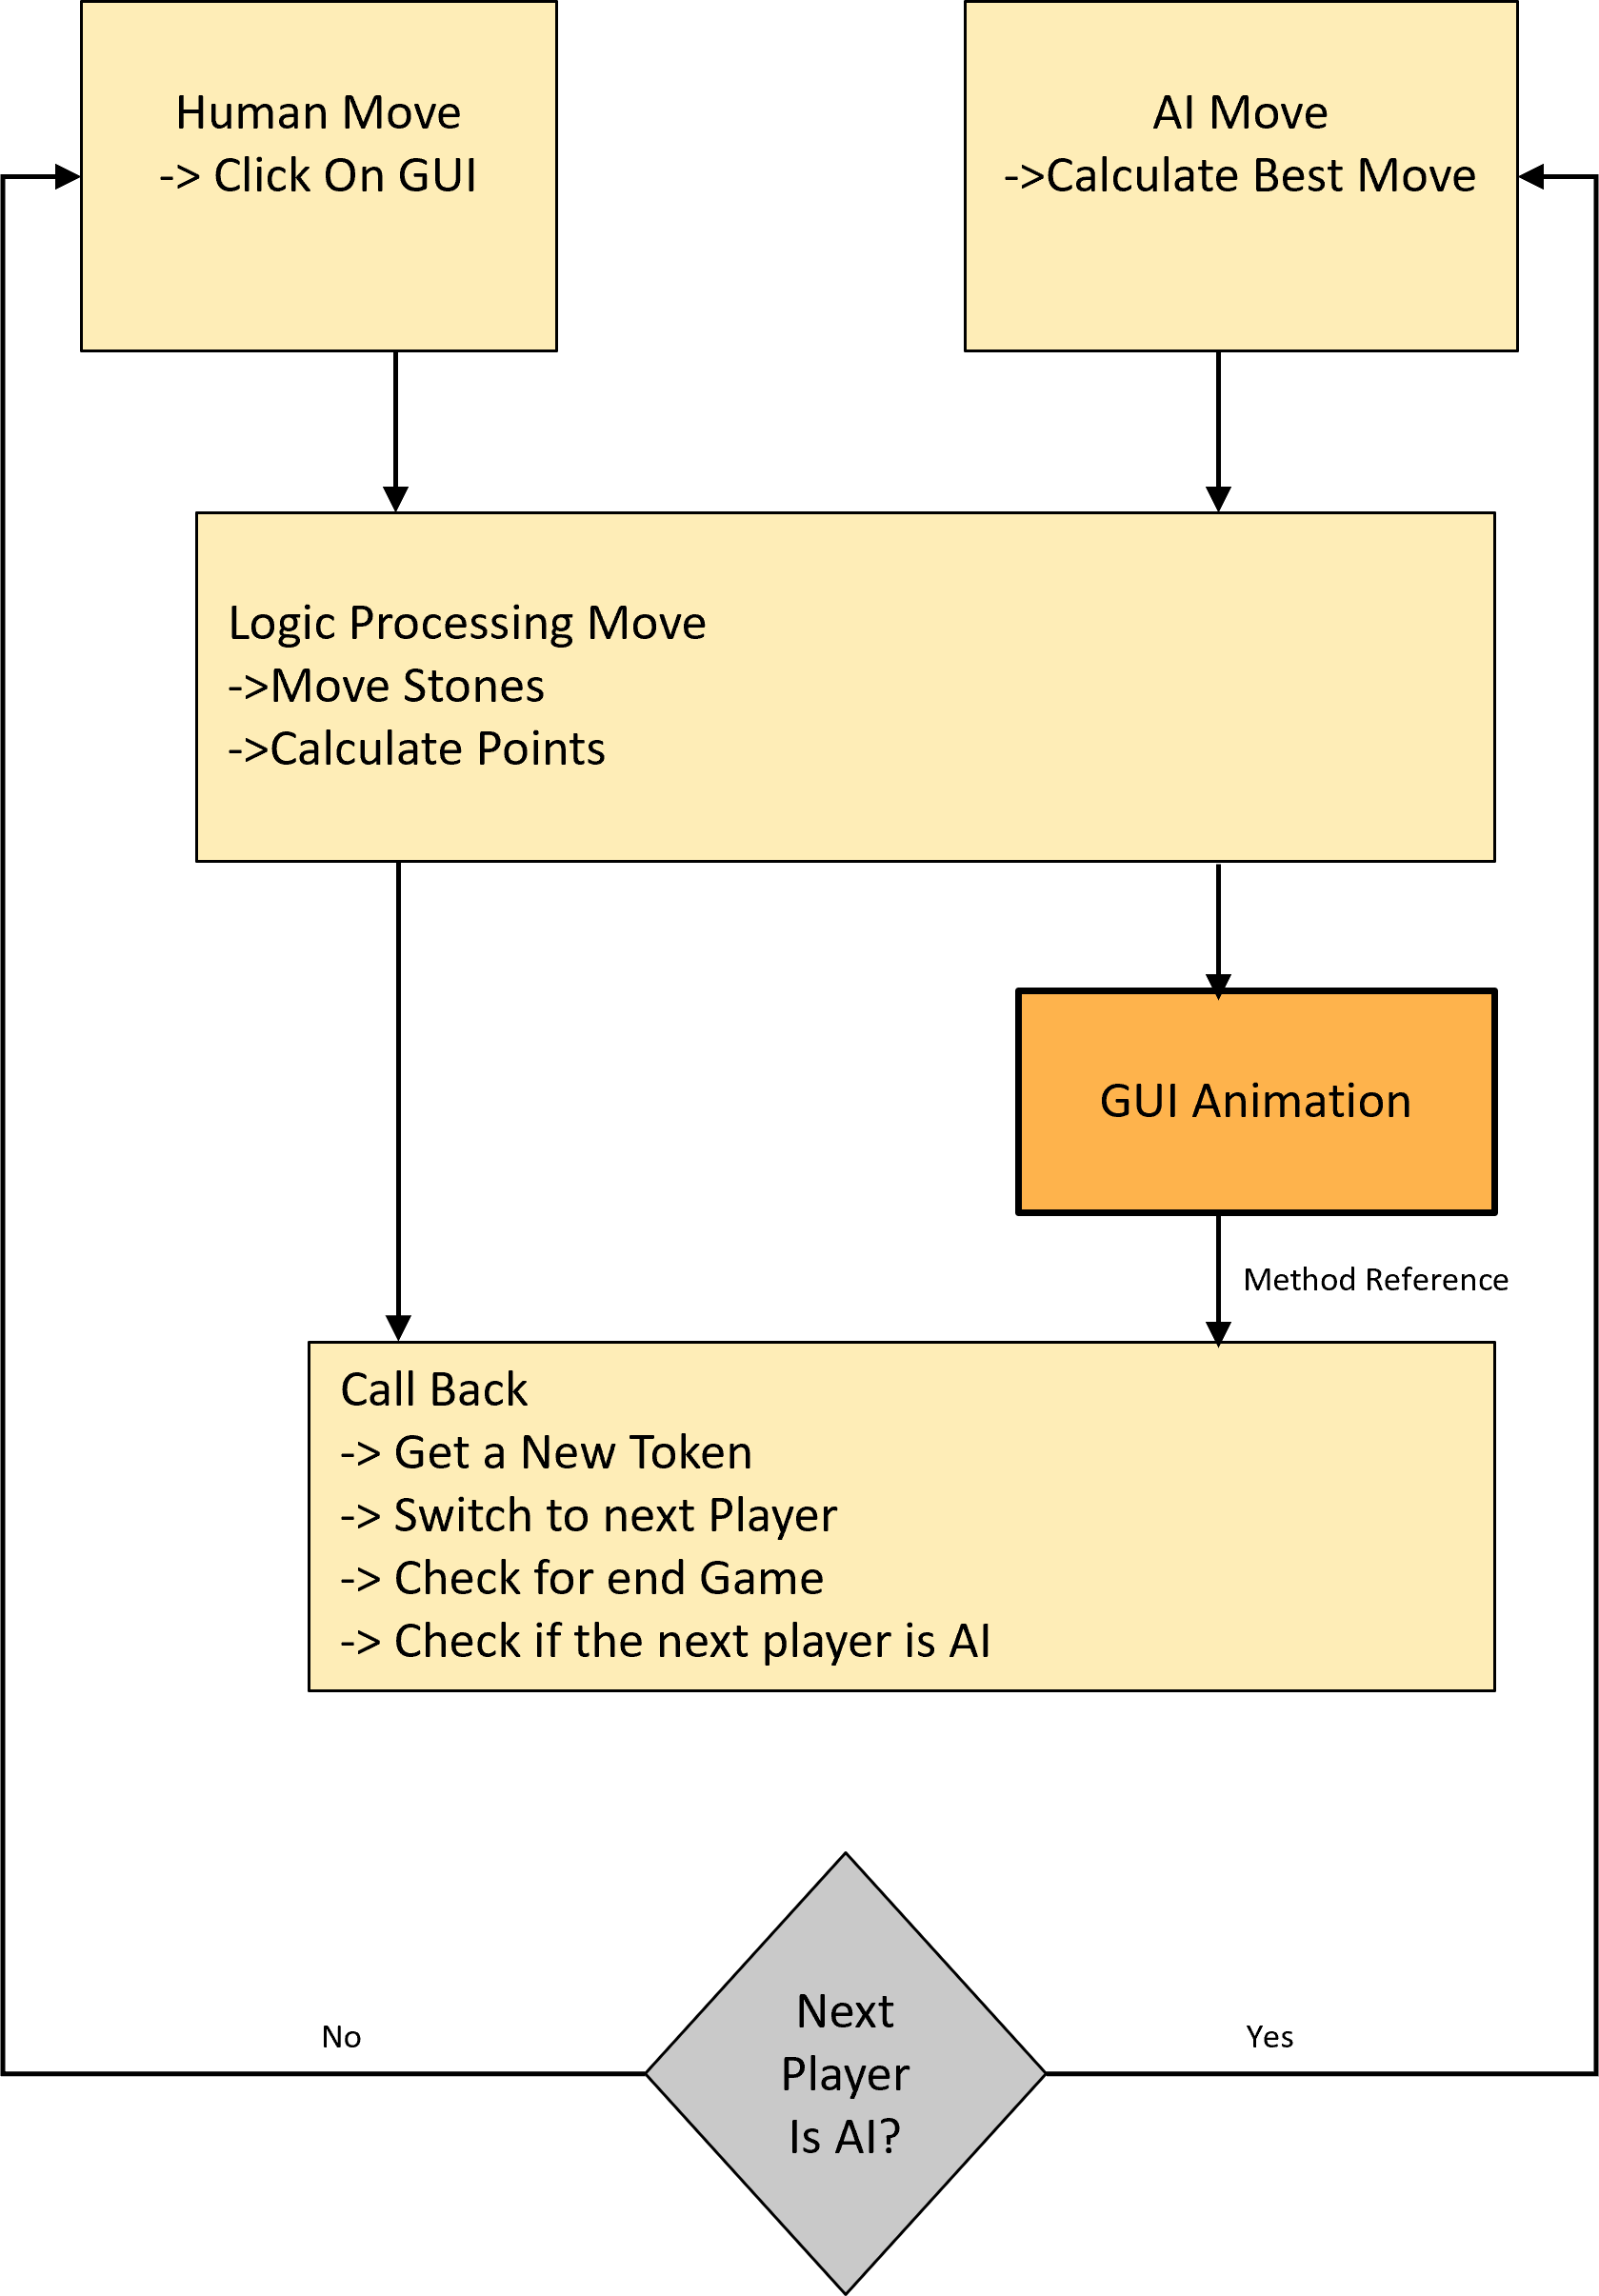
\includegraphics[width=0.6\textwidth]{image/StructureOfCallback}
	\caption{The Structure of callback function.}
	\label{fig:StructureOfCallback}
\end{figure}

    
\section{Program organization plan}

\begin{figure}[h]
	\centering
	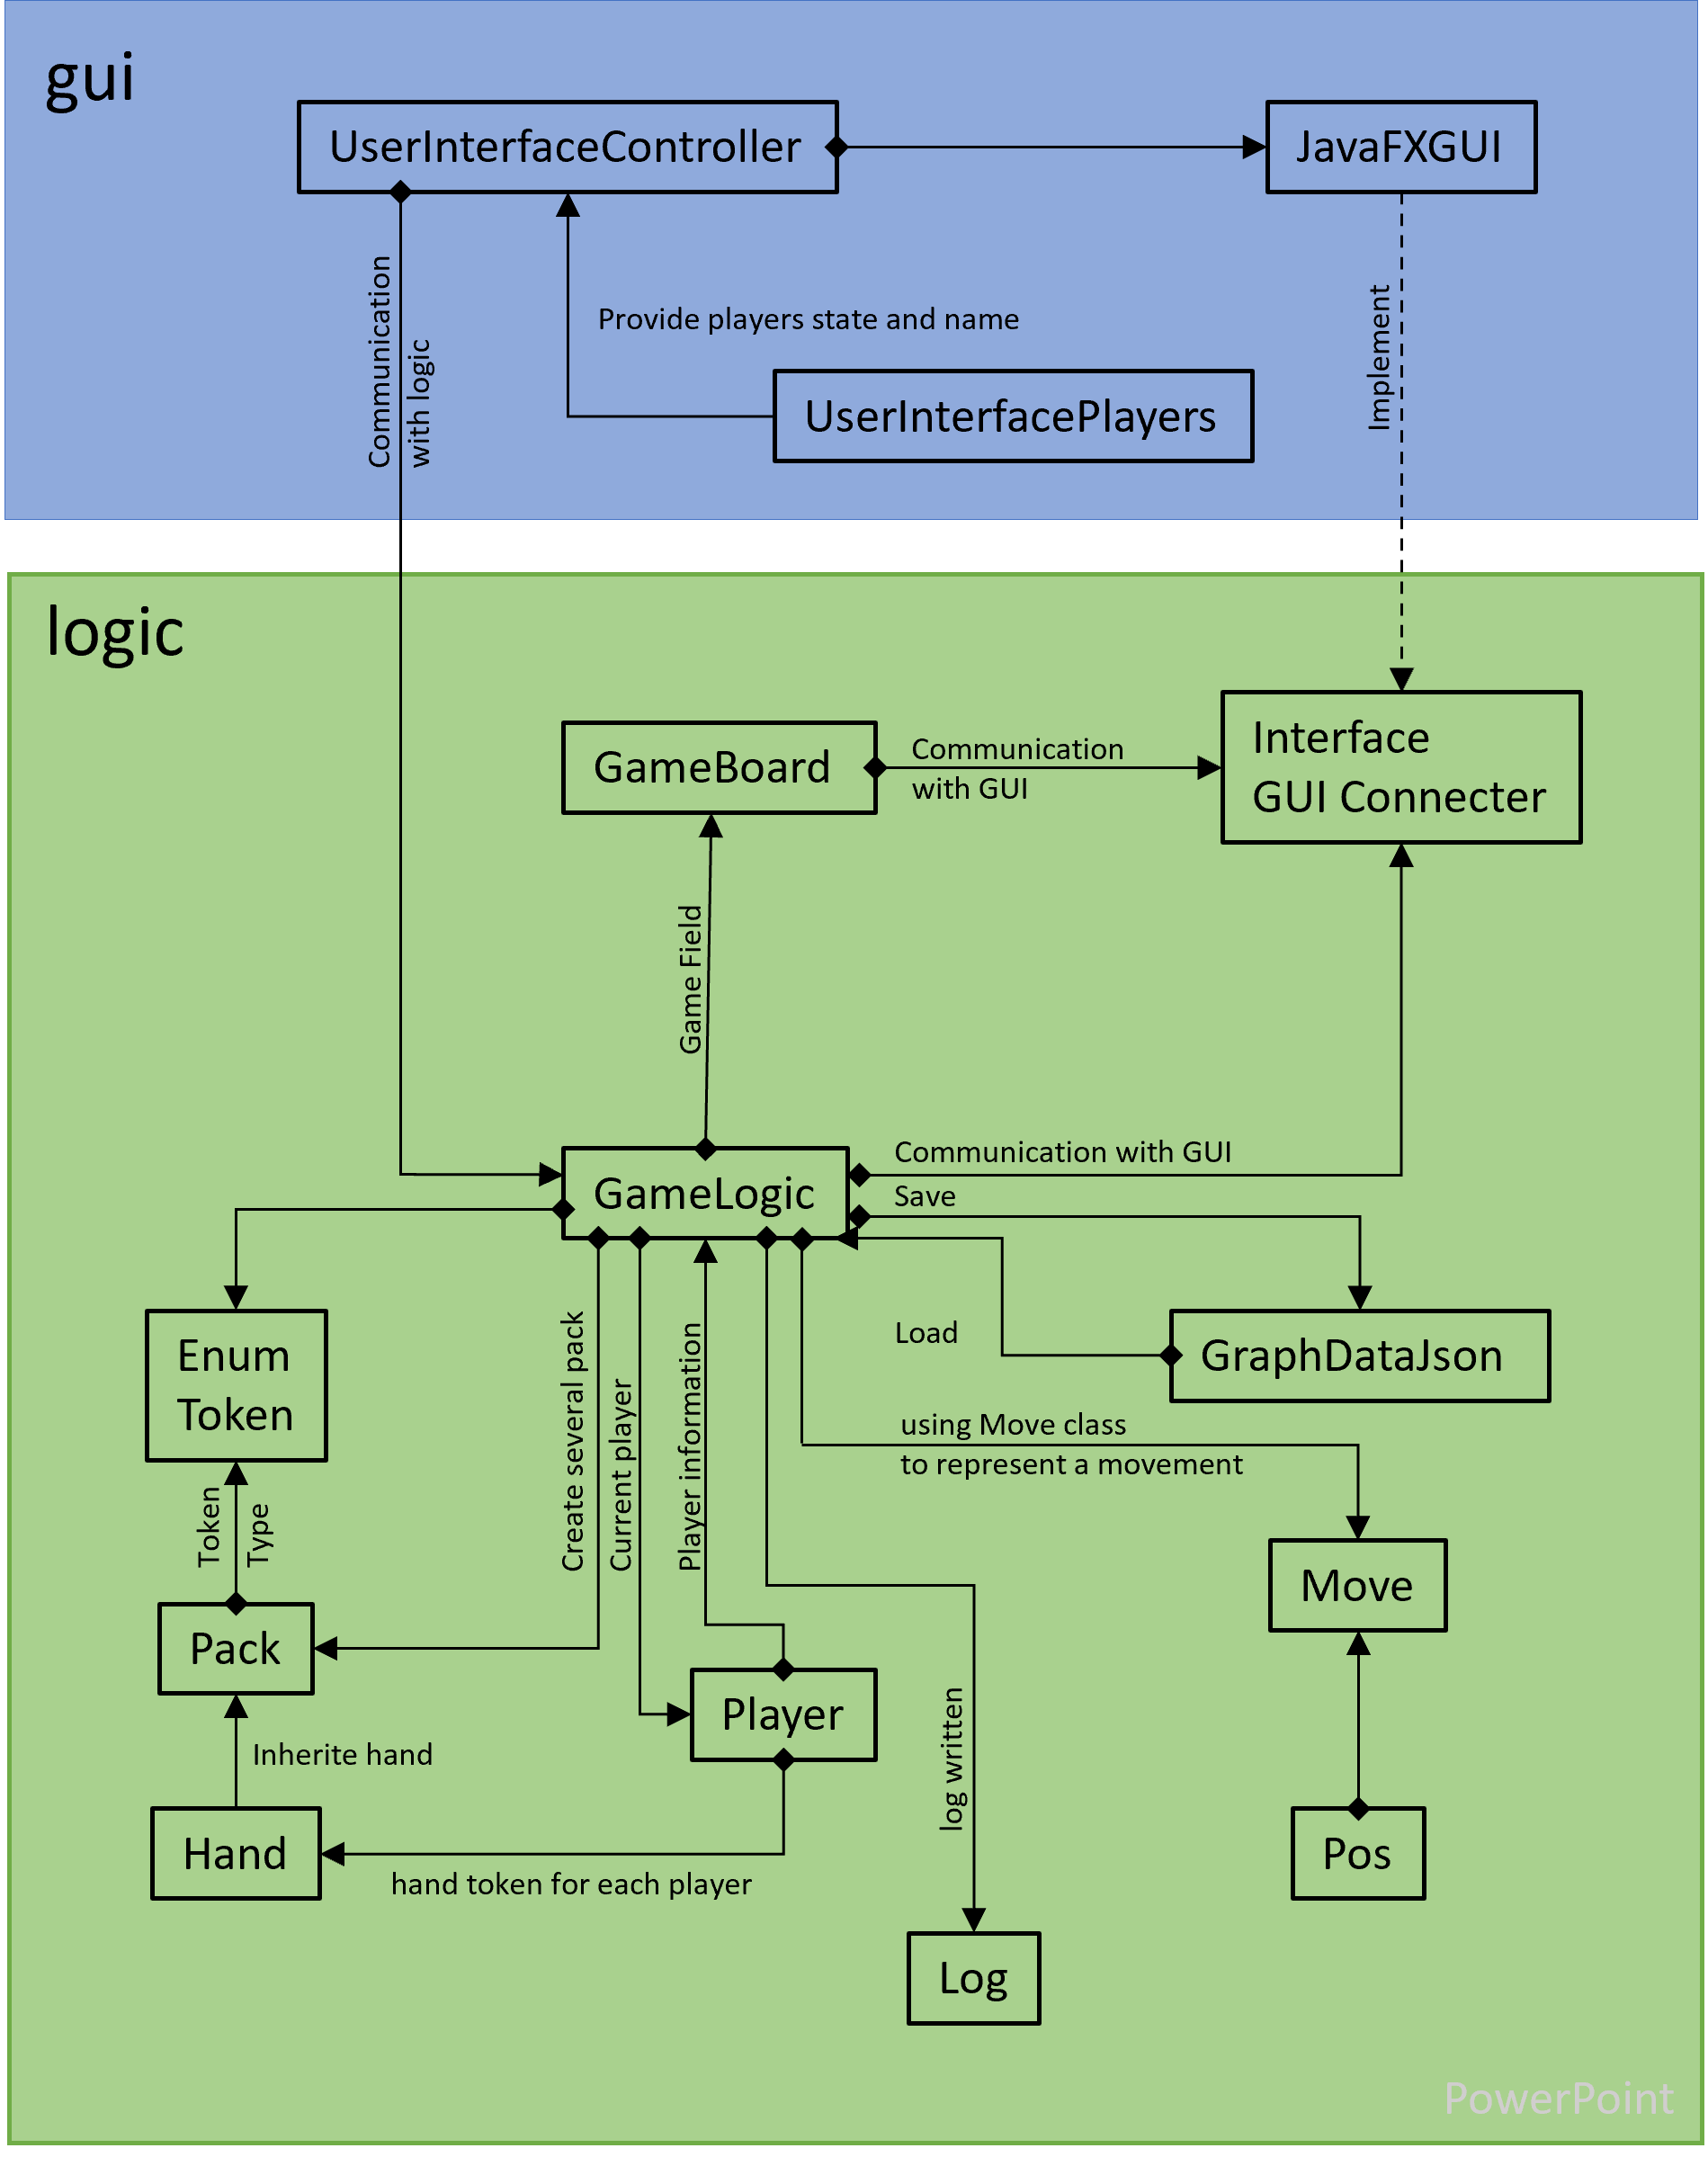
\includegraphics[width=0.8\textwidth]{image/diagram_1}
	\caption{The classes diagram}
	\label{fig:All classes diagram}
\end{figure}


\subsection{The package of GUI}

\subsubsection{UserInterface Controller and UserInterface Player}

The first FXML interface controller is responsible for the main scene and communicates with the logic package. Any performance of the users is exhibited on this primary User Interface, for example, players can operate the game, select the provided options on the menu bar, and observe the current game situation. 

For the second scene UserInterfacePlayer, it manages the initialization of the state of participants. Players can manually insert their names and decide which players will be played by the bot. 

With regards to the communication of these two windows as the Figure \ref{fig:guiPackage} below, the first interface establishes a reference of the second window in order to getter method to pass players' names and states to the main window. 
It can clearly conclude that it is a one-direction for passing information from the first scene to the second scene. 


\begin{figure}[h]
	\centering
	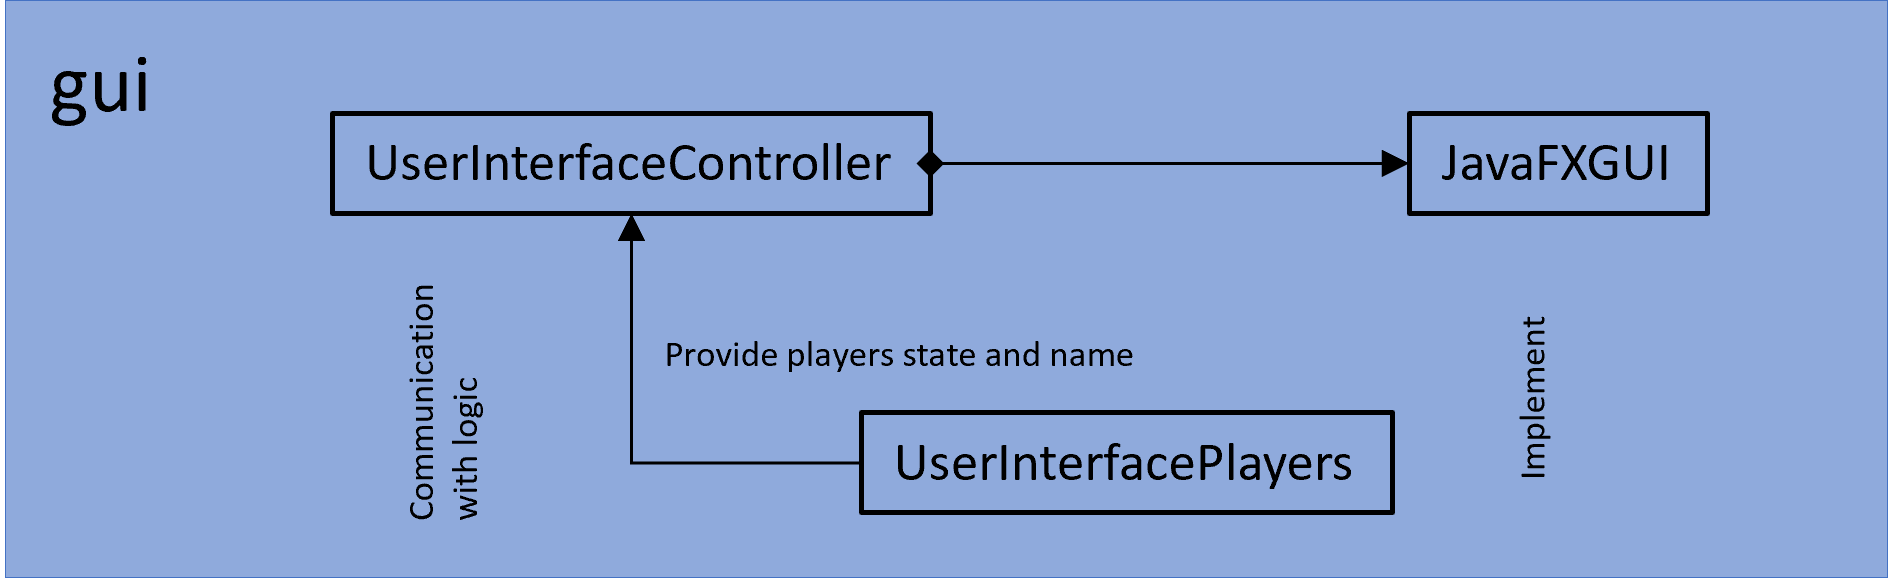
\includegraphics[width=0.8\textwidth]{image/diagram_2}
	\caption{The GUI package}
	\label{fig:guiPackage}
\end{figure}

\subsubsection{JavaFxGUI}
The aims of all the methods in JavaFxGUI allow the logic class to change the output GUI. In fact, the JavaFxGUI can be implemented by the class GUIConnector, which is being used in the logic package. For example, while the logic class needs to modify the chessboard by placing a symbol token, it is undoubtedly that the display of the interface also needs to update the game field simultaneously. 
Thus, the function of the class JavaFxGUI can be utilized for this purpose. 

\newpage
\subsection{The package of Logic}

\begin{figure}[h]
	\centering
	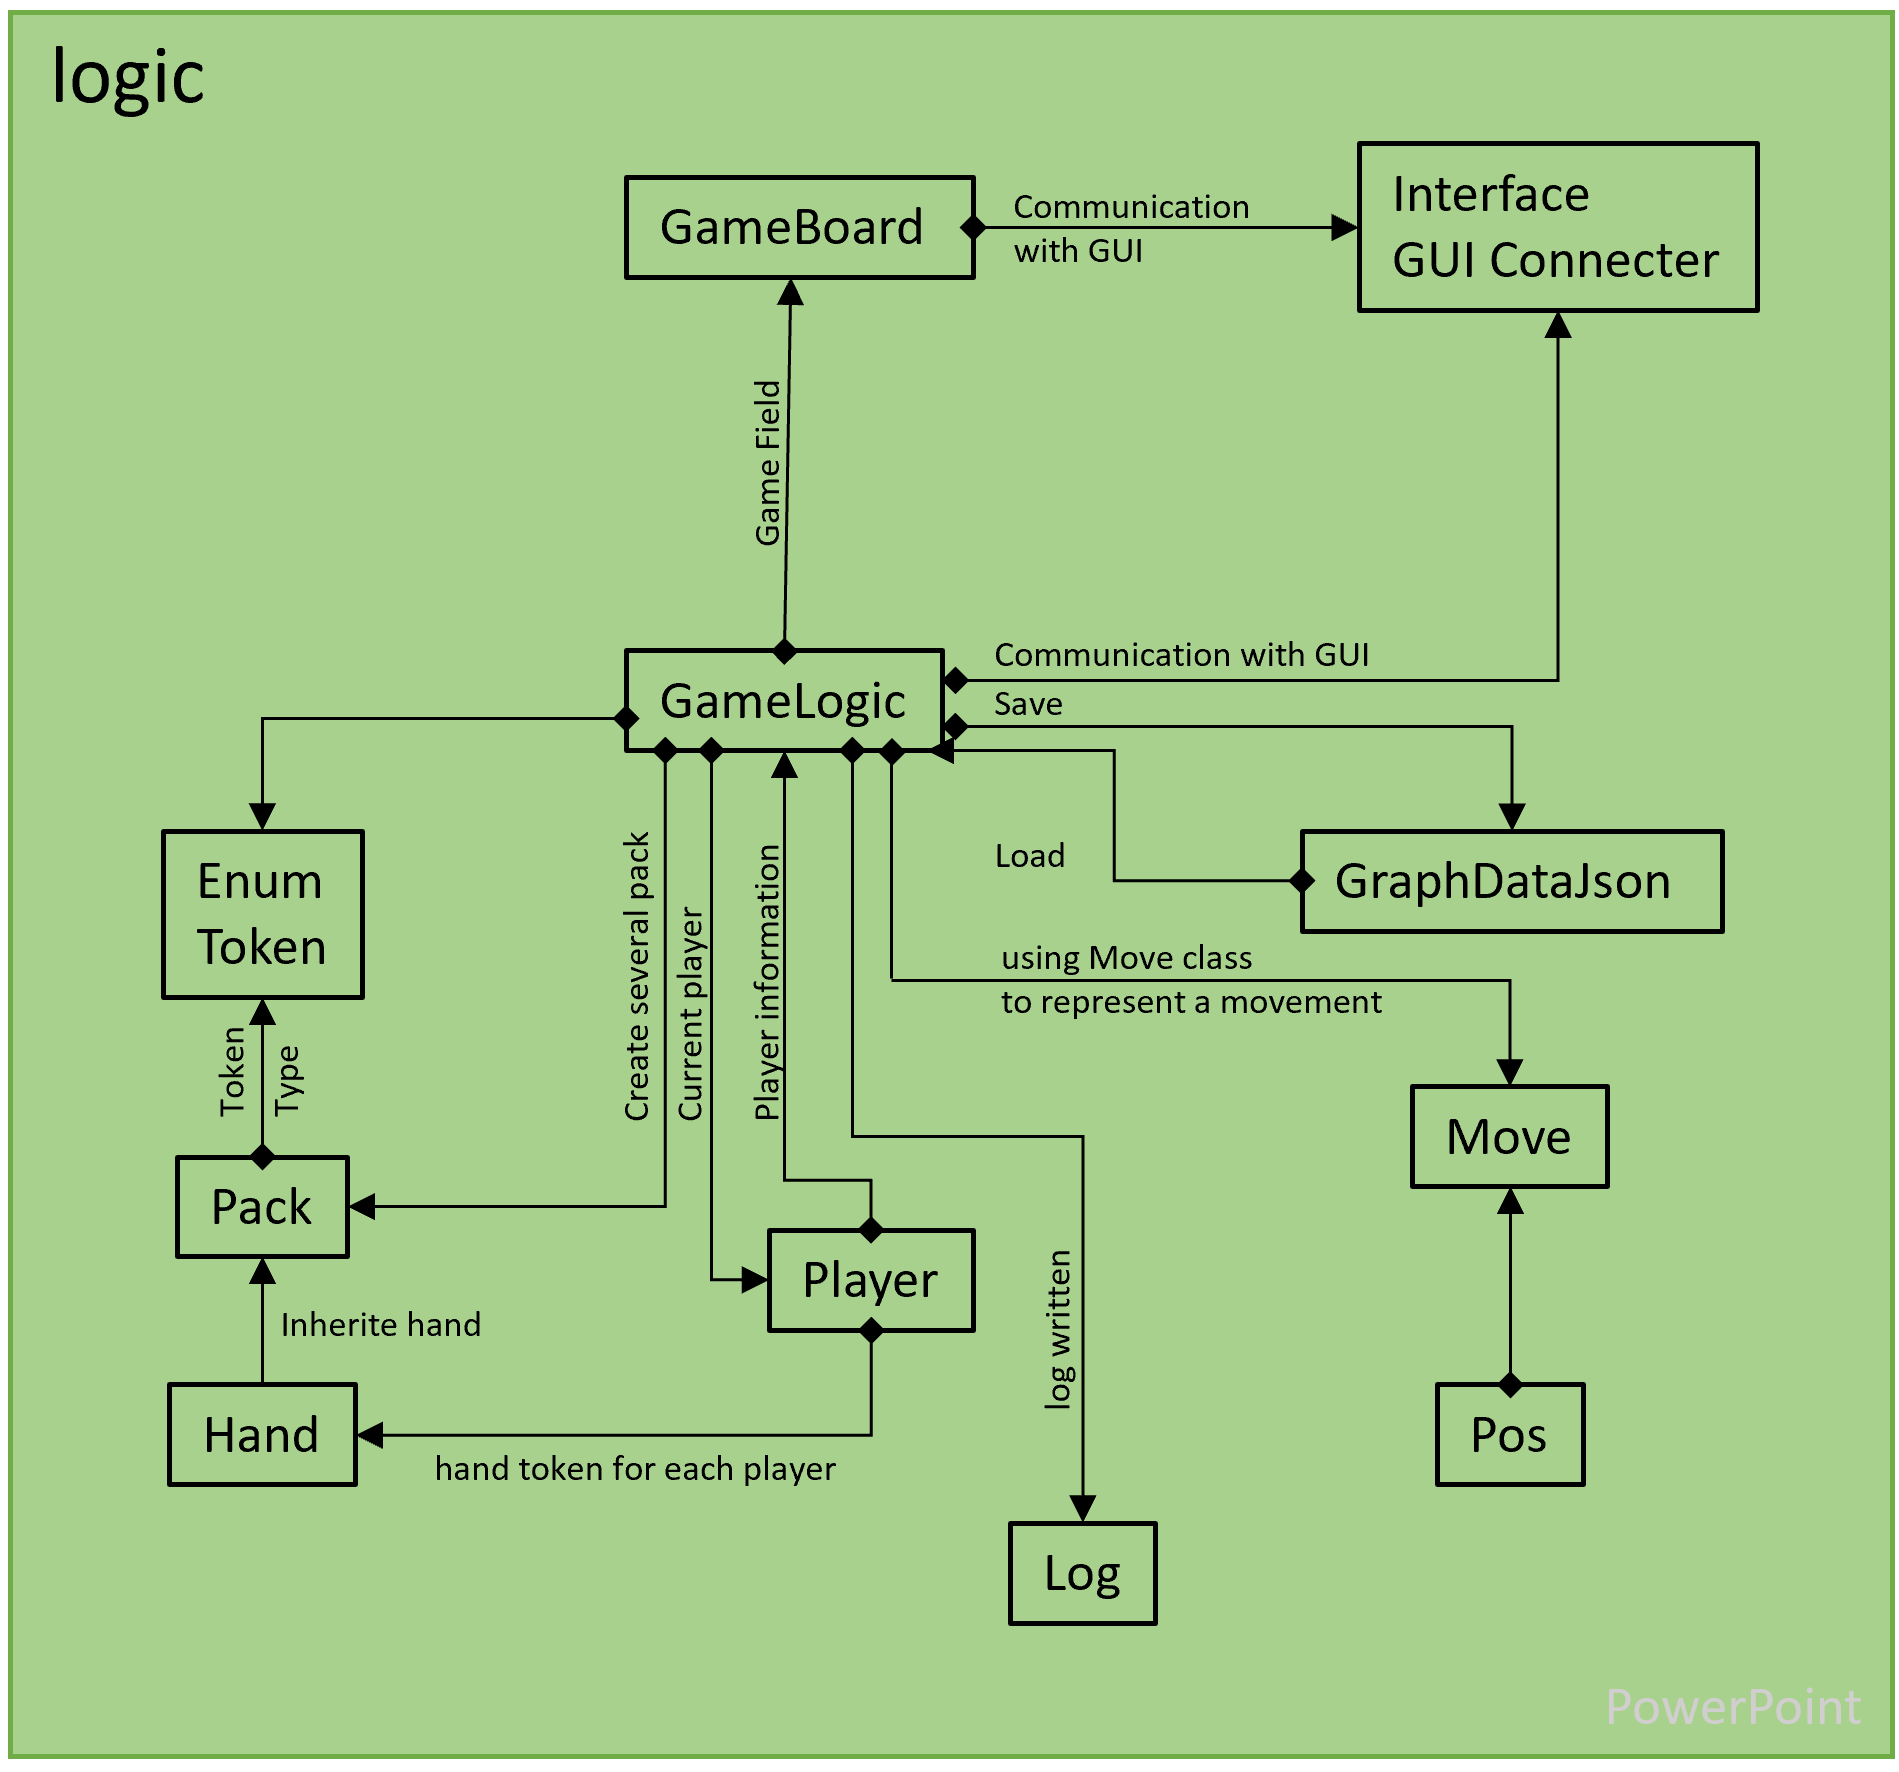
\includegraphics[width=0.8\textwidth]{image/diagram_3}
	\caption{The Logic package}
	\label{fig:logicPackage}
\end{figure}
\subsubsection{Game Logic}


The class Logic is mainly controlled the whole program of the game, the most important core class among it. All other classes will be implemented here and be integrated into the logic of the whole game such as the logic algorithm of the AI, the logic program to determine the winner, and the initialization of the whole game. 

From Figure \ref{fig:gameLogic} below, it is apparent to recognize that the class Logic also needs to communicate bidirectionally with other classes to update some features of the game.

In detail, the class logic frequently interacts with the class player to track the feature of the current player. And lead this feature to the GUI package to display on the main interface in order to become a condition, which is for the participant to realize who needs to play now.   

Additionally, the class Logic also produces an interaction with the class Pack to have a global constant of a full pack, which functions to count the number amount of tokens. Not only does a full pack of all tokens exist but also a pack keeping every action token is required in the program. 
While a token is being used, the token pack needs to be diminished as a used token each time.

Furthermore, as mentioned in the top description, the class Move and the class Position are also being used in some methods of analyzing AI movement.  As a tool, they are generated as an object corresponding to on their class type.


\begin{figure}[h]
	\centering
	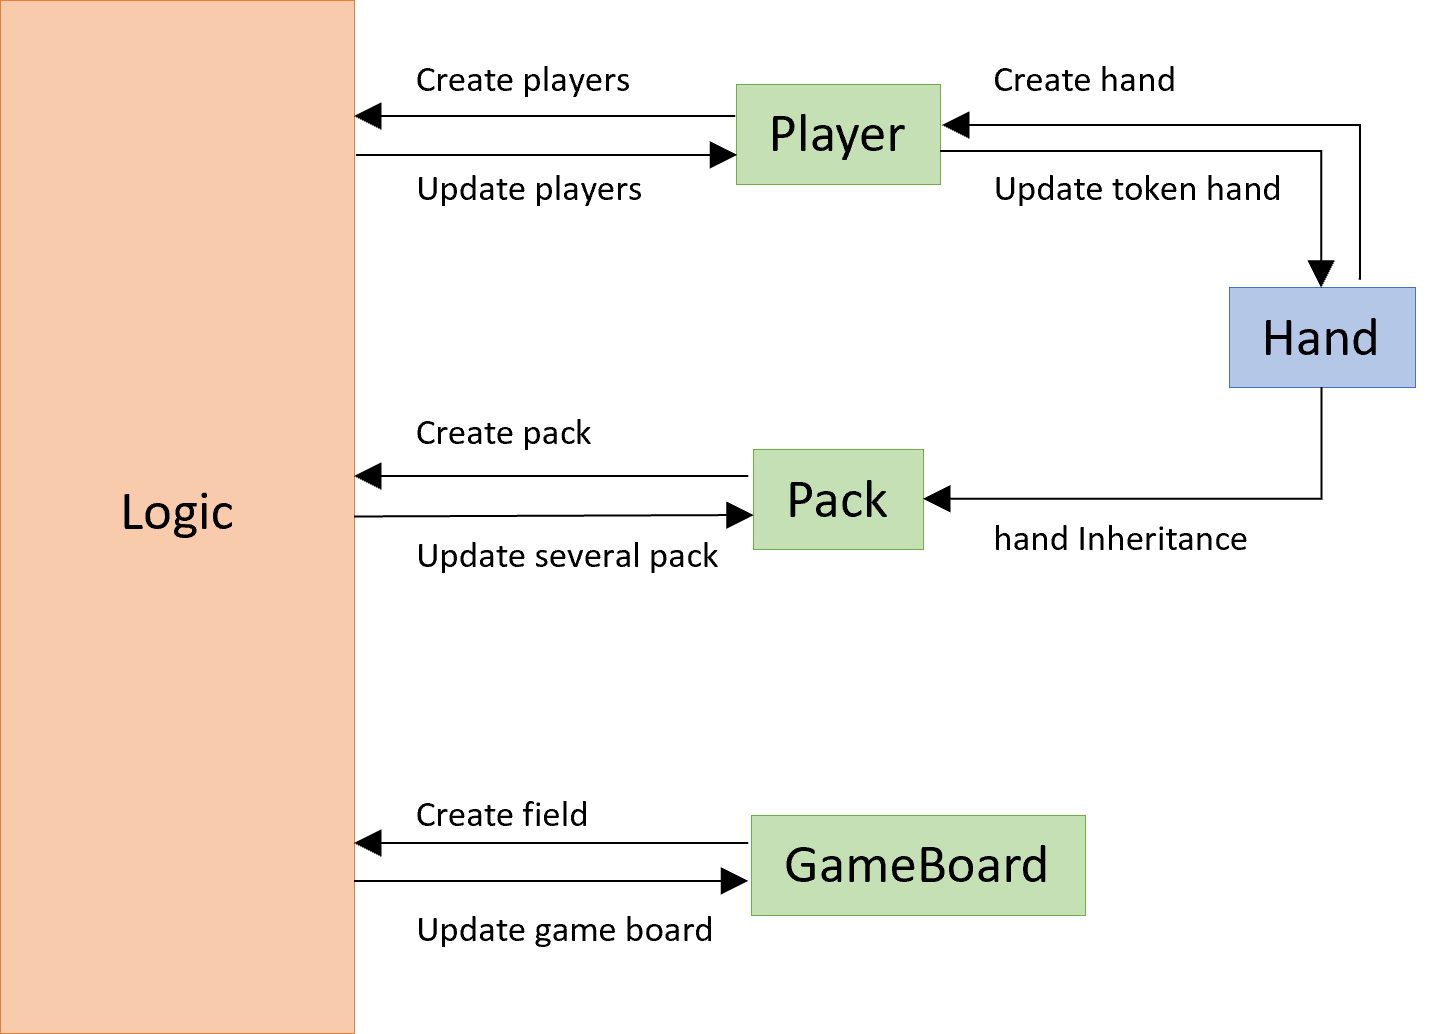
\includegraphics[width=0.8\textwidth]{image/diagram_4}
	\caption{The relationship between GameLogic class and other classes.}
	\label{fig:gameLogic}
\end{figure}


Here has two essential and noticeable developing logics that needs to be mentioned below:

\paragraph{Human} \mbox{}\\
Regards to the logic of the human player playing the game, a few coordinates of the game board and the player's hands are considered the fundamental gist. While a human player uses click or drag action to play the game, the coordinate of those actions needs to be recorded and passed to other functions to accomplish other aims.

\paragraph{AI logic}\mbox{}\\
In the AI logic, it is important to claim that there are some rules that existed in the game. As the turn is in AI, the idea for AI to pick up the best token to get the best score or even attempt to win the game has its own logical design.
In the developmental of our logical design, the two main types of token: Symbol token and Action token are introduced and follow the rules below:   


\begin{enumerate}
	\item\textbf{Winning a game by laying a line of six}\\
    The player should be able to use the token to complete six tokens in a line and win the game. 
This condition is the priority of winning the whole game. However, one thing that needs to realize is that the action token must always be utilized first and then the symbol token is the second option. 
	\item\textbf{Prevent another team to complete six}\\
Since another team has accumulated five tokens in a line on the chess board, the player should be aware of and use tokens to interrupt the possibility of winning the game for another team. Likewise, the action token must be used in advance. 
	\item\textbf{Achieve the best score}\\
	However, achieving the best score has a different arrangement that the symbol token must be considered first when the player has a symbol token on hand. The action token will only be considered when there is no line of six to be completed and there are no symbols token on the player's hand, 
	
\end{enumerate}



\subsubsection{Game board}

A class Game board is represented as a field generated by every token which has been arranged on the chess board. All the methods existing in this class are related to the changes in behaviour or some identified use. It is apparent to observe that the game board class is directly output to the logic class as the player drag and drops a token on the board or modifies some changes. 

\subsubsection{Player}

The class Player aims to create an object player in a game. The object of the player involves several attributes, for instance, the name of the participant, the active state, the AI state, and the hand token for the participant. 
In the constructor of the class logic, the player class can be implemented with the purpose of creating several players for game playing. And also the logic class can keep tracking the current player with the player object.    

\subsubsection{Pack and Hand }

According to the understanding of the game playing, a pack of storing tokens and a hand token of each player is an indispensable element in a game. Hence, with the help of many methods, the class logic can utilize the Class pack to insert, remove or increase tokens in a pack or player's hands. Moreover, because of the inheritance relationship of the class pack and class hand as shown in Figure \ref{fig:packAndHand} below, those methods in the pack class are also applicable to be utilized for hand class. 

\begin{figure}[h]
	\centering
	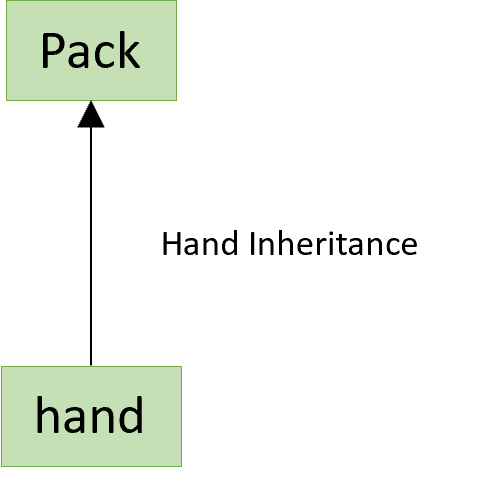
\includegraphics[width=0.3\textwidth]{image/diagram_5}
	\caption{Pack and Hand}
	\label{fig:packAndHand}
\end{figure}

\newpage
\subsubsection{Enum Token }

Regarding the Enum class Token, every token is numbered in an enum category. An advantage of sorting those tokens in the sequence is that other classes are able to invoke the specified token by an ordinal. The sequence of tokens is shown below Figure \ref{fig:enumToken}.

	\begin{figure}[h]
	  \centering
	  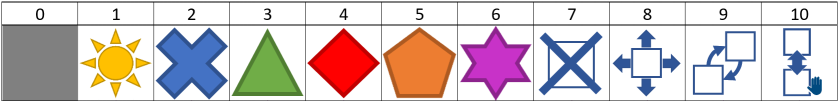
\includegraphics[width=0.8\textwidth]{image/sequenceOfEnumTokens}
      \caption{The sequence of Enum tokens}
	  \label{fig:enumToken}
    \end{figure}

\subsubsection{Move and Position}

The function of the class Move and the class Position is principally the same. Mostly they have a constructor which includes an object to record the necessary attribute and this object can be passed to any class which is required. Indeed, the class Move even contains a position object to perform the movement position as shown in Figure \ref{fig:moveAndPosition} below. Among the position object, it has two attributes x and y, which are the coordinate of the chess board.
  
\begin{figure}[h]
	\centering
	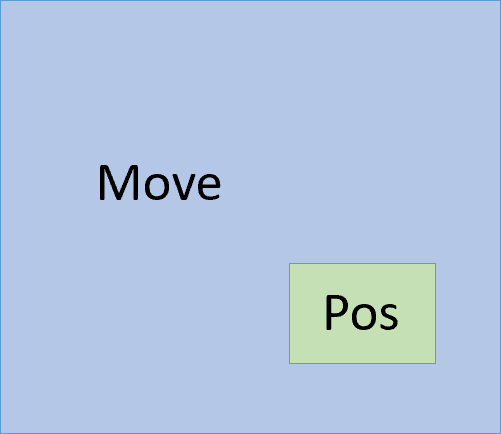
\includegraphics[width=0.3\textwidth]{image/diagram_6}
	\caption{The Move and Position class.}
	\label{fig:moveAndPosition}
\end{figure}


\subsubsection{GraphDataJson}

In this project, the conception of Save and Load is based on the JSON file. To parse a JSON file, GSON is chosen for implementation. And this class contains all information, which is necessary for generating an unfinished game that would be established as a variable in class logic. No matter which operation of Save and Load to use, both of them must through this variable to transform data. The process of transforming data is as below in Figure \ref{fig:GraphDataJson}.      

\begin{figure}[h]
	\centering
	
\includegraphics[width=0.6\textwidth]{image/diagram_7}
	\caption{The GraphDataJson class and GameLogic class.}
	\label{fig:GraphDataJson}
\end{figure}



\section{Files}

\subsection{Save and Load File}
A file existed for a game to record the game situation, and continuous playing of an unfinished game or a customized game can be executed. The file is written as a text by using GSON format to represent the whole game situation, just as the Figure \ref{fig: JSONFile} below. 


\begin{figure}[h]
	\centering
	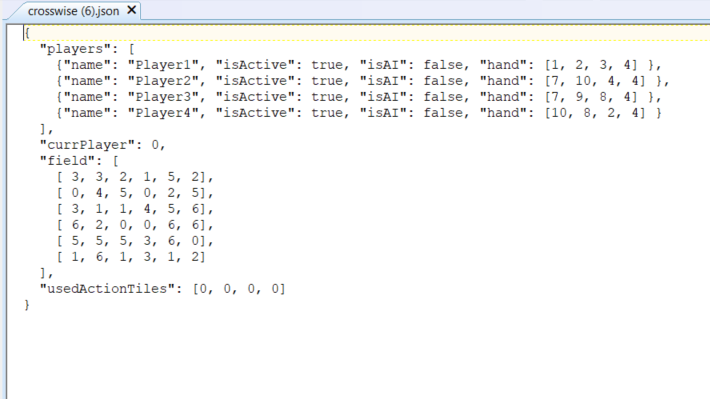
\includegraphics[width=0.8\textwidth]{image/JSON format}
	\caption{The representation of GSON}
	\label{fig: JSONFile}
\end{figure}


\subsubsection{Save}

In the program, the player class could provide the name of the player, active state, AI situation, and the hand token of this player and transfer them into text format.

Additionally, the current player and the field of the whole game board could be transformed into a number representation. Although the board tokens are presented as an enum element, in the board class, we create a method that can be transforming that enum element into an int representation. 

At last, this archive also must involve the list of the used action token, which can remind players of the amount remained number of the action token. The list of action tokens has already used the int array to track in the logic class.

Those transferring behaviors would need to use the getter methods of the class GraphDataJson to complete. 

The ultimate text representation is shown as Figure \ref{fig: JSONFile}.


\subsubsection{Load}

Likewise, loading a game with an archive, in which the file format is as the Figure \ref{fig: JSONFile}. And the recorded attributes must be bound with the attribute in the program.  With the purpose of assigning the value to the program attribute, the setter method of the class GraphDataJson could be used to set up. 

\subsection{Log File}

A log is written to a file so that the programmer can retrace the steps in the event of an unexpected program response. This file is overwritten or recreated each time the game is started. In the program, a class Log is created to use a logger object to log messages for a specific system or application component. Furthermore, a simple method "WriteToLog " is created in order to let Class logic implement and conveniently document when an event happens, for example, a player places a token on the board. Furthermore, there is also some situation when the game encounter a problem such as the no Token in the deck and the player could not have a new Token. The representation of the Log File is shown as Figure \ref{fig: logFile} below.

\begin{figure}[h]
	\centering
	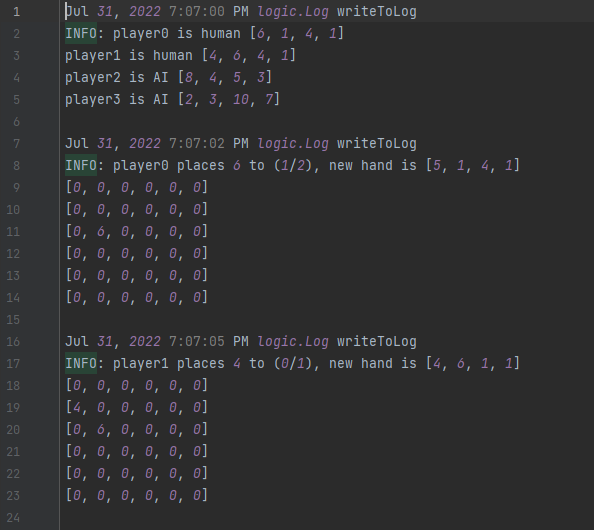
\includegraphics[width=0.8\textwidth]{image/logFile}
	\caption{The representation of Log file}
	\label{fig: logFile}
\end{figure}



\newpage
\section{Program testing}

\subsection{AI algorithm}
In this section of testing removing the action token for AI, there are three main essential to evaluate: Has six same tokens for the current team, prevent another team from reaching six tokens, and achieve the best score. Additionally, this testing includes external files. Follow the steps below: 

\begin{itemize}
	\item Check the folder "AI algorithm", and the subfolder "remove token".
	\item Select which teams: "Orange" and "Green".
	\item Each had three test cases. 
\end{itemize}


\subsubsection{Symbol Token}	

\begin{table}[h]
	\centering
	\begin{tabular}{p{7cm}@{\hskip 5mm}  p{7cm}} 
		\toprule
		Test case   & Result   \\ 
		\midrule
		\midrule
         While there are no action tokens on hand and the current team has a specific token to accomplish the six in a line, this specific token need to be chosen and placed where it should be. In fact, the coordinate of lacking the specific token must be empty as a condition. & The expectation is that the player could place the right token in the right place. And the result shows as expected. \\
		\midrule
	     While there are no action tokens on hand and the opposite team has a specific token to cease the six tokens accomplished by the opposite team  this specific token need to be chosen and placed where it should be. In fact, the coordinate of lacking the specific token must be empty as a condition. & The expectation is that the player could place the right token in the right place to interrupt the opposite team win a game. And the result shows as expected. \\
		\midrule
		 Generally speaking, when the player has a series token on hand and achieving the best score is the priority of the game. And the symbol token needs to accomplish this goal.  The test case is that the current player will use one of the symbols tokens to achieve the best score for his/her team. & The expectation is that the difference between the two team scores should be as large as possible. And the result is shown as expected even though there is no chance to reduce the opposite team.    \\
		\bottomrule
	\end{tabular}
\end{table}

\newpage
\subsubsection{Remove Token}	

\begin{table}[h]
	\centering
	\begin{tabular}{p{7cm}@{\hskip 5mm}  p{7cm}} 
		\toprule
		Test case   & Result   \\ 
		\midrule
		\midrule
		The current team has a chance to complete six same tokens. Use remove token to remove the unique Token on a line that has accumulated five same tokens.  & The expectation is that the unique token has been removed and returned back to the players' hands. And the result shows as expected. \\
		\midrule
	    The opposite team has a chance to complete six same tokens. Use remove token to remove one of the same Tokens on a line that has accumulated five same tokens. & The expectation is that the coordinate of the removed token is smaller the further it is up and the further it is to the left. And the result shows as expected.  \\
		\midrule
	    The current has a full action token on hand including one remove token, which has the smallest index on the hand. The test case is that the current player will use this removed token to achieve the best score for his/her team. & The expectation is that the difference between the two team scores should be as large as possible. And the result is shown as expected even though there is no chance to reduce the opposite team.     \\
		\bottomrule
	\end{tabular}
\end{table}

\newpage
\subsubsection{Shifter Token}

\begin{table}[h]
	\centering
	\begin{tabular}{p{7cm}@{\hskip 5mm}  p{7cm}} 
		\toprule
		Test case   & Result   \\ 
		\midrule
		\midrule
	     The current team has a chance to complete six same tokens. Use shift token to shift the unique Token on a line that has accumulated five same tokens to the empty cell on the line.  & The expectation is that the unique token has been founded on the board and shifted to the empty cell of the line in order to complete six tokens. And the result shows as expected. \\
		\midrule
		The opposite team has a chance to complete six same tokens. Use a shifter token to shift one of the same Tokens on a line that has accumulated five same tokens to the empty cell which has the smallest row and column. & The expectation is that the coordinate of the shifter token start from the first same token of the line and the target empty coordinate is smaller the further it is up and the further it is to the left. And the result shows as expected.  \\
		\midrule
		The current has a full action token on hand including one shifter token, which appears on the smallest hand index. The test case is that the current player will use this shifter token to achieve the best score for his/her team. & The expectation is that the difference between the two team scores should be as large as possible. And the program will find the token that can cause the smallest effect on the current team and the most serious losing point to the opposite team. And the result is shown as expected. \\
		\bottomrule
	\end{tabular}
\end{table}

\newpage
\subsubsection{Exchange Token}

\begin{table}[h]
	\centering
	\begin{tabular}{p{7cm}@{\hskip 5mm}  p{7cm}} 
		\toprule
		Test case   & Result   \\ 
		\midrule
		\midrule
		The current team has a chance to complete six same tokens. Use Exchange token to Exchange the unique Token on a line that has accumulated five same tokens to the position which acquired this unique token.  & The expectation is that the unique token has been founded and switched to the position in which the line has had five same tokens.If there are two needed tokens appear on board, then the program chooses the smallest row and column index. And the result shows as expected. \\
		\midrule
		The opposite team has a chance to complete six same tokens. Use Exchange token to exchange one of the same Tokens on a line that has accumulated five same tokens to the token which is located as close as the left top corner. & The expectation is that one of the exchanging tokens is decided as the lowest index on the line no matter what row or column. And another exchanging token is the token that appears closest to the left top of the chess board. And the result shows as expected.  \\
		\midrule
		The current has a full action token on hand including one Exchange token, which has the smallest index on the hand. The test case is that the current player will use this Exchange token to achieve the best score for his/her team. & The expectation is that the difference between the two team scores should be as large as possible. And the program will find the token that can cause the smallest effect on the current team and the most serious losing point to the opposite team. And the result is shown as expected even though there is no chance to reduce the opposite team.     \\
		\bottomrule
	\end{tabular}
\end{table}

\newpage
\subsubsection{Replace Token}
In the test case of the Replace token, only two considerations are being tested. The "Achieve the best score" test is not unable to implement in the case of the Replace tokens. Because of the characteristic of the Replace token, it needs to contain at least one symbol token on the token hand. However, according to the designing logic, achieving the best score always start from the symbol token.

\begin{table}[h]
	\centering
	\begin{tabular}{p{7cm}@{\hskip 5mm}  p{7cm}} 
		\toprule
		Test case   & Result   \\ 
		\midrule
		\midrule
    	The current team has a chance to complete six same tokens. Use Replace token to switch the needed Token on a line that has accumulated five same tokens to the cell which needed this special token.  & The expectation is that the unique token has been switched with the token, which appears on the gap of the line and it returns back to the player's hand. And the result shows as expected. \\
		\midrule
    	The opposite team has a chance to complete six same tokens. Use Replace token to switch one of the same Tokens on a line that has accumulated five same tokens with one token on hand, which is not related to the line. & The expectation is that the index of the replaced token from hand is as low as possible. And this token must be different from that special token on the line. And another switching token also has the lowest index of column and row.  And the result shows as expected.  \\
		\bottomrule
	\end{tabular}
\end{table}

\newpage
\subsection{Test Load}

\begin{table}[h]
	\centering
	\begin{tabular}{p{7cm}@{\hskip 5mm}  p{7cm}} 
		\toprule
		Test case   & Result   \\ 
		\midrule
		\midrule
	    Test if the current player is AI, and check if the program is able to execute perfectly. A created testing file in the folder "Test Load". After creating a new game, select the Load menu button and choose "Current Player is AI".  & The expectation is that the program will still work perfectly and the AI player will start to place tokens on the board. And the result shows as we expected.  \\ 
	    \midrule
	    Test if the current player is human, and check if the program is able to execute perfectly. A created testing file in the folder "Test Load". After creating a new game, select the Load menu button and choose "Current Player is Human".  & The expectation is that the program will still work perfectly and the human player can start to play the game. And the result shows as we expected.  \\ 
	    \midrule
	    Test if all participants are AI, and check if the program is able to execute perfectly. A created testing file in the folder "Test Load". After creating a new game, select the Load menu button and choose "All AI player".  & The expectation is that the program will still work perfectly. Each AI participant places their desired token on the chess board correctly. And the result shows as we expected.  \\ 
	    
		\bottomrule
	\end{tabular}
\end{table}

\newpage
\subsection{Test Save}

The purpose of this test case is that a game has been started to play and store as a JSON file by saving. And those saved files need to be invoked and loaded to ensure the game situation is displayed as the same. Thus, there are few external files that have been created in advance.\\  


Following the step below to load the specific test case :

\begin{itemize}
	\item Check the folder "Test Save".
	\item Select the specific case.
\end{itemize}


\begin{table}[h]
	\centering
	\begin{tabular}{p{7cm}@{\hskip 5mm}  p{7cm}} 
		\toprule
		Test case   & Result   \\ 
		\midrule
		\midrule
    	From JSON format, a hand token contains null. & The expectation is that the GUI will display the null expression on this hand. For example. there is no image on the required position. However, the result did not show as expected. The position of the null still has an image on it. This image is the same as the image of the one smaller index position. But one noticeable point of the null token is that even if the null position has an image, the human player cannot do any action in this area. Hence, the null position will not cause a NullPointer exception at last. \\ 
    	\midrule
        Test a saved file in two players. When a game with only two players is stored in JSON format, the third player and fourth player have not been activated. Then their hand also has no Token. Nevertheless, the syntax of the token hand will be stored as empty. This test case needs to ensure those empty hands could be transferred and bounded. & The expectation is that due to the third player and fourth player do not attend the game, the game must not show the GUI display. And also the turn of the player will only switch between first and second. 
        The result is entirely shown as expected.  \\
        \midrule
       Test case for customized used action token. The display of the remaining action token must not as the same as the content of the used toke array. & The expectation of this test case is that there is one action token is being used for Shifter, Exchange, and Replacer. But the removed token stays the same. Therefore, the display number of the action token must be {3, 2, 2, 2}. In comparison, the customized used action token array is {0, 1, 1, 1}. Fortunately, the results show as expected. \\
		\bottomrule
	\end{tabular}
\end{table}

\newpage
\subsection{The restriction of different tokens and the duration of highlighting the test }

\subsubsection{Remove Token}	
\begin{table}[h]
	\centering
	\begin{tabular}{p{7cm}@{\hskip 5mm}  p{7cm}} 
		\toprule
		Test case   & Result   \\ 
		\midrule
		\midrule
		While the chess board does not contain any token, and the human player tries to use the Remove token function. & The expectation of this test case is that the human player could not select Remove token on hand. And the result of this testing shows precisely what we have expected. The human player cannot click the Remove token when there is nothing to remove from the board.  \\ 
		\midrule
		A Remove token is being triggered and observe the changes on the player's hand. & The expectation is that the player's hand will not get a new token and simply just get the token, which is removed from the board. And the final result shows the expectation perfectly.  \\
		\midrule
		Test duration of remove token. The removed token should be marked and the marking sign should only exist for a short time. After beginning a game, click on the options menu to decide the duration time of highlighting. & The expectation is only the highlighted region of the removed token on board should fade out. And the marked region of the removed sign should not change and stay as normal. And the result shows as expected. \\
		\bottomrule
	\end{tabular}
\end{table}
\newpage
\subsubsection{Shifter Token}

\begin{table}[h]
	\centering
	\begin{tabular}{p{7cm}@{\hskip 5mm}  p{7cm}} 
		\toprule
		Test case   & Result   \\ 
		\midrule
		\midrule
		While the chess board does not contain any token, and the human player tries to use the shifter token function. & The expectation of this test case is that the human player could not select the Shifter token on hand. And the result of this testing shows precisely what we have expected. The human player cannot click the shifter token when there is nothing to select and shift.  \\ 
		\midrule
		Test duration of shifter token. The shifter token should be marked and the marking sign should only exist for a short time. After beginning a game, click on the options menu to decide the duration time of highlighting. & The expectation is both coordinates of start and target on board should fade out. And the marked region of the shifter sign should not change and stay as normal. And the result shows as expected. \\
		\bottomrule
	\end{tabular}
\end{table}

\newpage
\subsubsection{Exchange Token}

\begin{table}[h]
	\centering
	\begin{tabular}{p{7cm}@{\hskip 5mm}  p{7cm}} 
		\toprule
		Test case   & Result   \\ 
		\midrule
		\midrule
		While the chess board does not contain any token, and the human player tries to use the Exchange token function. & The expectation of this test case is that the human player could not select Exchange token on hand. And the result of this testing shows precisely what we have expected. The human player cannot click the Exchange token when there is nothing to switch.  \\ 
		\midrule
		While the chessboard only contains a symbol token, and the human player tries to use the Exchange token. & The expectation is that the Exchange token cannot be triggered on hand.  And there is a warning alert shown up to remind players cannot use the Exchange tokens.\\
		\midrule
		Test duration of Exchange token. The exchange token should be marked and the marking sign should only exist for a short time. After beginning a game, click on the options menu to decide the duration time of highlighting. & The expectation is both coordinates of first changing and second changing on the chess board should fade out. And the marked region of the exchange sign should not change and stay as normal. And the result shows as expected. \\
		\bottomrule
	\end{tabular}
\end{table}

\newpage
\subsubsection{Replace Token}

\begin{table}[h]
	\centering
	\begin{tabular}{p{7cm}@{\hskip 5mm}  p{7cm}} 
		\toprule
		Test case   & Result   \\ 
		\midrule
		\midrule
    	While the chess board does not contain any token, and human players try to use Replace token function. & The expectation of this test case is that the human player could not select replace token on hand. And the result of this testing shows precisely what we have expected. The human player cannot click the Replace token when the board is empty.  \\ 
		\midrule
		Test duration of Replace token. The replacement token should be marked and the marking sign should only exist for a short time. After beginning a game, click on the options menu to decide the duration time of highlighting. & The expectation is both coordinates of the first changing on hand and the second changing on the chess board should fade out. And the marked region of the Replacer sign should not change and stay as normal. And the result shows as expected. \\
		\bottomrule
	\end{tabular}
\end{table}



\newpage

\subsection{During the game}

\begin{table}[h]
	\centering
\begin{tabular}{p{2.5cm}@{\hskip 5mm}  p{5cm}@{\hskip 5mm} p{6.5cm}} 
	\toprule
	error message   & cause      & corrective action  \\ 
	\midrule
	\midrule
    Exchange token cannot be used & Player may not use Exchange Token when there are less than two tokens on the board & Reselect an available token on his hand  \\

	\bottomrule
\end{tabular}
\end{table}

\begin{figure}[h]
	\centering
	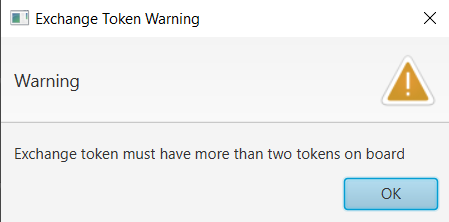
\includegraphics[width=0.6\textwidth]{image/ExchangeToken}
	\caption{Exchange Token Warning}
	\label{fig:ExchangeTokenWarning}
\end{figure}

\newpage
\subsection{End the game}

\begin{table}[h]
	\centering
	\begin{tabular}{p{7cm}@{\hskip 5mm}  p{7cm}} 
		\toprule
		Test case   & Result   \\ 
		\midrule
		\midrule
		While no token on the board, the player holds four action tokens. There is a created testing file in the folder "During the game". After creating a new game, select the Load menu button and choose "No available token".  & The expectation is that the current player can still click or drag the token on hand in attempting. However, a warning alert pops out that No available token for the player, and please start a new game.  The result is shown as expected because the current player cannot do anything and the game should be restarted.   \\ 
		\bottomrule
	\end{tabular}
\end{table}

